\section{Executive Summary Overview}
This notebook is the documentation of our FTC 4290 team and our journey starting from the trip back from the 2014 FIRST World Championships up until the preparation for this seasons 2015 FIRST World Championships.  We started off with summer projects to strengthen our weaknesses and focused on our technical, marketing and outreach planning so that we were ready when school started and the FTC season kicked off.  This season, we participated in and hosted several scrimmages, competed in two qualifiers, the Alamo Regional and the FTC South Super Regionals.  Along the way, we all worked together and focused on the engineering design, build, outreach activities, practice \& more practice, fundraising and all the learnings, frustrations and joy that our team and the robot has experienced together.\\

At the 2014 World Championships, our team observed best practices from the World Champion FTC teams. We talked, interacted and watched the teams using Mecanum drive technology and Field Oriented Drive. We cheered for the teams with fantastic strategy and superior autonomous programs. These teams inspired us to strive and become one of the teams competing on the 2014-2015 Edison and Franklin.  We are proud to represent the South, from Texas, as one of the 128 teams in the World Championships on the Edison Field and aspire to compete on the DaVinci field in the finals.\\

Over the summer, we worked with our mentors to organize into subteams, working on build technologies, drive train strategies, autonomous coding, marketing and recruiting. We assessed using LabView vs RobotC and made the decision to move to RobotC. Our goal was to put together a design, build it and provide the drivers with enough time to practice before qualifiers. We used a new design methodology and focused on rapid prototyping because our two seniors had very strong CAD and build skills. We continued to support our outreach programs with our SMART Camps and Robot demos and put a plan in place to recruit Freshmen to our team. Our fundraising was successful enough that we were able to buy all the game pieces for this season’s game.  This enabled our drivers to practice and our team to host scrimmages with other FTC teams.  We focused on continuous improvement and had GBU (Good, Bad and Ugly) reviews after every scrimmage and competition to prioritize improvements in robot, programming, outreach and presentation.\\

To complement and facilitate communications and project management, we evaluated on-line methods including Trello to help improve our communications and project management skills. We decided after beta testing Trello, over the summer, we would use it for the 2014-2015 season.  This notebook is the product of many, many hours of hard work to modify the Trello application.  The work is detailed in lists highlighted in the “notebook” section of this notebook.  Our team believes that without Trello, we would not have had the success that we did on and off the field.  The communications and project management pitfalls common in previous seasons were mostly mitigated with Trello and direction from our team coach.\\

We are proud of our Robot and Award performances this year. Table 1 below summaries our successes and route that we took to get to the World Championships.\\

\begin{figure}[H]
	\centering
	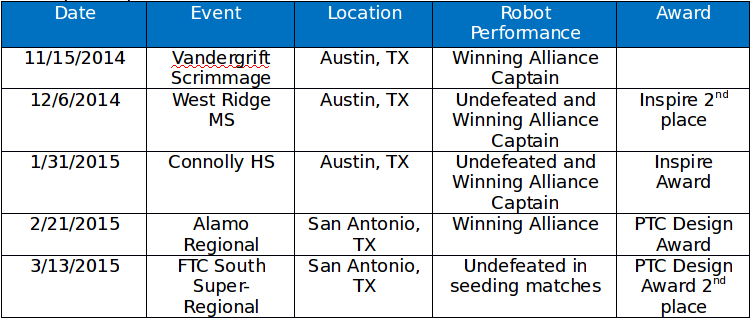
\includegraphics[width=\linewidth]{events}
	\caption[]{FTC 4290 Events for the 2014-2015 Season}
	\label{fig:events}
\end{figure}


We have enjoyed working together this season using the new design methodology and Trello.  We have grown together as a team, enjoying fostering and growing the Austin FTC community.  We look forward to seeing friends and meeting new ones at the upcoming 2015 World Championships in St. Louis.\\

\newpage

\section{Notebook Organization - Trello tool}
Notebook, communication and project management are a key factor to success for any project. We had previously used a blog entry system and understood the pros and cons of keeping a notebook in that format.  This summer, the team started to evaluate and use new tools including Trello that is based on project management and tasks. It was encouraged by our industry mentors from National Instruments and IBM.  After our evaluation, we made the decision to proceed and have not regretted it.\\

Trello is a free project management tool that improves and enhance our team communications and documentation. We ran a parallel effort to use our regular notebook process and Trello until mid July. Our evaluation of Trello was favorable and we decided to use Trello for our project/tasks and were pleased with its success as a communication/documentation tool.  Our team members and our coach are all smartphone savvy and particularly liked being able to access the “notebook”, discuss, communicate and make decisions instantaneously.\\

We have clarified through the FTC Q\&A that using Trello is an acceptable form for Notebook and used the Trello tools and our programmers on the team enhanced the tools to enable printing of this notebook today.  Below is the ruling from USFIRST on using the Trello tool for this notebook.\\

\begin{figure}[H]
	\centering
	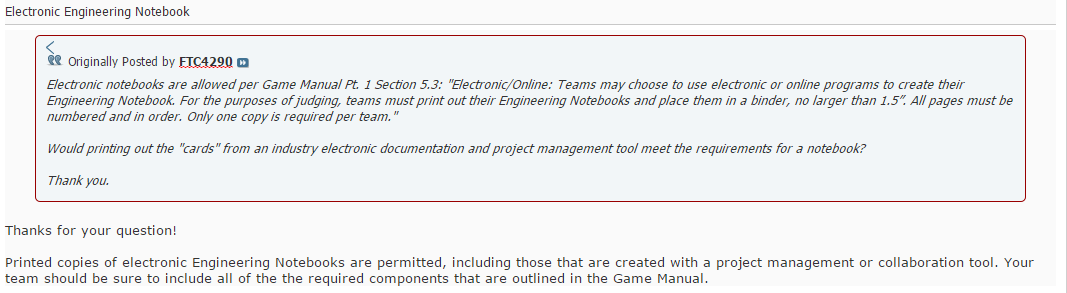
\includegraphics[width=\linewidth]{ruling}
	\label{fig:ruling}
\end{figure}

Trello is able to time date stamp and log in all the thoughts/comments and work efforts of every member of our team. It can keep lists/tasks, host files, pictures, spreadsheets, links to other sites and tools, all in one easy to access place. As such, our notebook moved from a date/time based organization to a project/tasked based effort.  This enabled our busy mentors to quickly review our projects and help guide progress when it was convenient for them on their desktop, laptop, tablet or smartphone.\\

Our team members believe that Trello was integral to the success of our team by improving our project management and communication.  It has enhanced the chance of success by enabling 24x7 communication and documentation with pictures, links, videos posted right into the task card. We highly recommend Trello as a communication and documentation tool and have one team member focused on developing an interface to better comply with FIRST notebook requirements.  This notebook is the result of our team working together and applying each member's individual skills to accomplish team goals.\\

\clearpage
\newpage

\section{How to access our Trello notebook (in real time!)}
\begin{figure}[H]
	\centering
	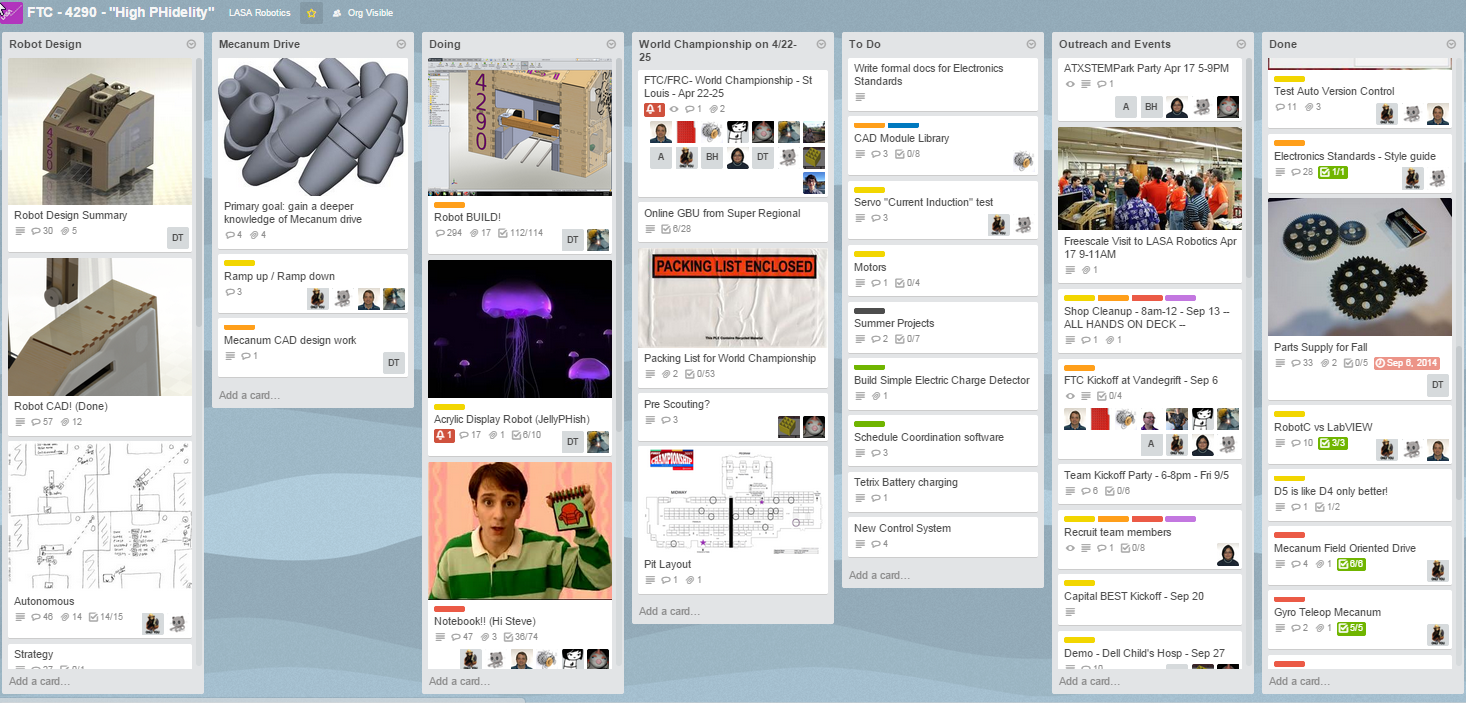
\includegraphics[width=\linewidth]{board}
	\caption[]{FTC 4290 Trello board - 4/18/2015}
	\label{fig:board}
\end{figure}

To log onto our Trello account from a laptop or mobile phone and access our individual cards...
\begin{enumerate}
\item Navigate to \url{https://trello.com}
\item Click "Log In" in the top-right corner
\item Login with username "lasajudge1" and password "purplehazed"
\item Click the board named "LASA - 4290 - HiPHidelity"
\item {\bf Explore the board!} (Please refrain from editing the board, but feel free to look around.)
\end{enumerate}

\clearpage
\newpage

\section{Team Overview}
\subsection{Team Mission Statement}
The Team mission is to inspire young people to be science and technology leaders, by engaging them in exciting mentor-guided, student-based programs that build science, technology engineering and math skills, that inspire innovation, and foster well-rounded life capabilities including self-confidence, communication, integrity and leadership.

\subsection{LASA Robotics Association Mission Statement}
The mission of the LASA Robotics Association is to support the LASA Robotics Team in developing and enhancing their skills and education to apply their knowledge, creativity, and intellect through a robotics competition format. The Association also serves as a conduit to facilitate community outreach, encourage entrepreneurial development, and provide community service opportunities.

\subsection{Team Origin}
The LASA Robotics team was formed in 1993 from students at LASA and LBJ High schools and is located in Austin, TX. LASA is the Magnet school in the Austin Independent School District, housed on the same campus as the 98\% minority composition LBJ High School. This “dual school, one voice” format allows the LASA Robotics Team to be very diversified in both student makeup and educational backgrounds.  The team was originally formed to compete in the BEST Robotics Competition (1995), MATE, and TCEA Robotics, the team now primarily competes in the FIRST Tech Challenge (FTC) and FIRST Robotics Competition (FRC).  We use FIRST competitions to hone in our critical thinking; improve our engineering skills in a fun environment, celebrating teamwork while competing.\\

LASA Robotics has a rich history with FIRST Robotics, starting in 2000 with the formation of FRC 418 and then with FTC 4290 in the 2010-2011 season and then starting FTC 5998 in the 2012-2013 season.  We serve as a breeding ground for future inventors and engineers, but we also give other motivated students the opportunity to experience a well-rounded STEM education. We have over 400 Alumni, many have studied in the engineering and science fields and are successful in industry or research fields. Appendix A lists our FIRST Awards and Achievements.   The coach of the LASA Robotics team has always been Mr. Anthony Bertucci. This season the coach for FTC 4290 is Gerry Cocco, a SW Programmer and Project Manager and our mentors are Cathy Cocco, a veteran in Technical Marketing, Janet Asghar who has been a World FTC judge and other engineers from industry including Cruz Monreal, a LASA Robotics Alumni from Silicon Labs and Adrian Knots \& Chris Rake from National Instruments.  We enjoy the support of the LASA Robotics Association which helps manage the team’s busy outreach schedule and tirelessly fundraises on behalf of the team.\\

\subsection{Team Organization}
The LASA Robotics Team is comprised of FRC 418 and FTC 4290 and FTC 5998.  In 2014-2015, we have 76 members that are registered to participate with 26 freshman on the team and 18 girls.  Every year, the team elects their leaders to help guide the team.  The FTC team roles this year are Drivers/Operators, Build, Programming, Notebook, Marketing, and Artistic Design.  For competitions, we also organize the scouting and presentation teams.  Students in each role could and did participate in multiple groups.  Besides the official team leadership, we encourage team members to form impromptu groups to accomplish specific tasks supporting robot demos, repairs and other smaller projects that need to get done.\\

As we are a magnet high school with students from all over Austin, many of our students are dependent upon the late school buses to get them home from after school activities.  This requires that students meet after school from 3:45PM to 6PM on Monday - Thursdays.  Many of our students don’t get home until past 7PM on the weekdays that the team meets.  Our meeting and work schedule also dictate that we have mentors that can support this schedule, limiting the industry employed mentors that have the flexibility to work with the team.\\

\begin{figure}[H]
	\centering
	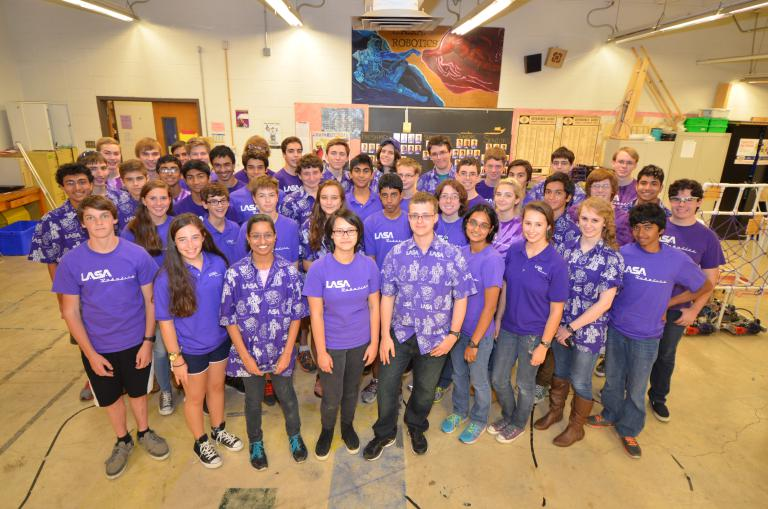
\includegraphics[width=\linewidth]{teamorg}
	\caption[]{Our team, 2014-2015}
	\label{fig:team}
\end{figure}

\clearpage
\newpage

\subsection{Current Team Status}
There are currently 76 members on the team, a 60+\% increase from 3 years ago. The team has overcome many challenges associated with rapid growth.  We are still working towards building student leadership and becoming better organized to more efficiently manage the students on our team.  Our goal is to provide all team members with a rewarding, interesting, and educational experience without exceeding our budget. Almost one quarter of the students are on the free and reduced lunch program and require scholarships for individual expenses which include travel, snacks and team shirt costs. LASA Robotics does not limit the size of the team nor require applications to join, keeping our financial goals and needs a moving target.\\

FTC 4290 is comprised of upperclassman from the LASA Robotics team.  In prior years, the two FTC teams were comprised of both freshman and upperclassman.  This year, in order to give freshman the chance to “roll up their sleeve” and not just watch and learn with the upperclassmen, we had all the freshman join the FTC 5998 team in Fall 2014.  Every team member from FTC teams then had the option to move to the FRC 418 team in the spring when the FRC team kicked off.  As a result, the FTC 4290 is a subset of the LASA Robotics team and the team bios included below are the main team members focused on this year’s FTC challenge.\\

\clearpage
\newpage

\subsection{Team Biographies}
\begin{figure}[H]
	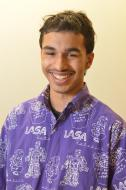
\includegraphics[width=0.2\linewidth]{ehsan}
\end{figure}
\subsubsection{Ehsan Asdar - Junior - Programmer} 
{\bf My role on the team}: Programming lead for FTC, Social Media for FTC 4290

{\bf Why I joined Robotics}: I joined the team due to previous interest in robotics from programs in elementary/middle school. I worked extensively with basic LEGO Mindstorms in those programs, but never was exposed to the more advanced programming and intense competition that FIRST Robotics programs provide.
	    
{\bf What career/job/studies I intend to pursue}: I intend to pursue a career in Computer Science and Electrical Engineering.
	
{\bf Thing I enjoy most about Robotics \& FIRST}: Watching the robots come to life for the first time after a long build and code season is the most rewarding part of robotics. Other than that, I really enjoy the collaboration aspect, where our subteams - drive, build, programming, marketing, etc. - all have to work toward a common goal.  The way the FIRST competitions are built require the team to have structure and organization, get things done in a timely manner and collaborate. Since I am on programming, I especially enjoy the software aspect which is basically "taking a giant oddly-shaped piece of metal and making it do something".

\begin{figure}[H]
	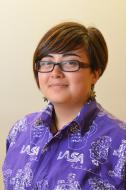
\includegraphics[width=0.2\linewidth]{julia}
\end{figure}
\subsubsection{Julia Cocco - Junior - Project Coordinator / Notebook}
{\bf My role on the team}: Marketing Lead

{\bf Why I joined Robotics}: I joined Robotics because my brother was on the team. Ever since I attended the 2009 FRC World Championship at the Georgia Dome, I knew that I just had to be a part of what was going on. Otherwise I felt like I'd be missing out! 

{\bf What career/job/studies I intend to pursue}: Industrial Engineering, Business Management, Event Coordination, Marketing, or Hospitality. My dream job is to help coordinate the FIRST World Championship! 

{\bf Thing I enjoy most about Robotics \& FIRST}: Celebrating the achievements of the next generation of engineers.

\begin{figure}[H]
	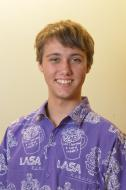
\includegraphics[width=0.2\linewidth]{blake}
\end{figure}
\subsubsection{Blake Hance - Junior - Driver} 
{\bf My role on the team}: I am the driver on FTC 4290.

{\bf Why I joined Robotics}: I liked the idea of being given a chance to solve a challenge by making a robot, and it seemed like there are a lot of things you can learn through a robotics club that you couldn't learn elsewhere as a high school student.

{\bf What career/job/studies I intend to pursue}: I plan on studying chemistry, more specifically organic chemistry or biochemistry, and I want to get a research job in that field.

{\bf Thing I enjoy most about Robotics \& FIRST}: I really enjoy the atmosphere at competitions. We work on our robot for months and we finally get to competition and we get to see how well it performs against all the other robots that other teams have toiled over. The sense of accomplishment at having all that preparation come together and competing with a bunch of other people who have done the same thing is very rewarding.

\begin{figure}[H]
	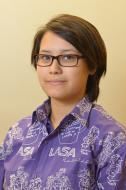
\includegraphics[width=0.2\linewidth]{kyla}
\end{figure}
\subsubsection{Kyla Hayworth - Sophomore - Operator} 
{\bf My role on the team}: Operator/secondary driver

{\bf Why I joined Robotics}: I was on an FLL team when I was in middle school and I saw LASA demoing one of their robots at an invitational. Those robots were so big that I was curious enough to join once I entered high school.

{\bf What career/job/studies I intend to pursue}: Architecture or electrical engineering

{\bf Thing I enjoy most about Robotics \& FIRST}: The sense of community is overwhelming when I walked into my first competition. Not only were there people that were enthusiastic about robots, but they were friendly and have made robotics about more than just the robot for me. 

\begin{figure}[H]
	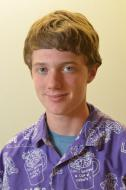
\includegraphics[width=0.2\linewidth]{jackson}
\end{figure}
\subsubsection{Jackson Hughes - Junior - Driver} 
{\bf My role on the team}: I am the coach for the drive team.

{\bf Why I joined Robotics}: I joined robotics because I wanted to be part of a group of people that are all interested and enjoy STEM activities, and robotics takes these activities and makes them even more fun by putting it into an interactive and entertaining competition like scenario.

{\bf What career/job/studies I intend to pursue}: I most likely will pursue an engineering career and studies after high school. 

{\bf Thing I enjoy most about Robotics \& FIRST}: I enjoy the exciting competitions and all the great people involved in FIRST since it really brings forth a great environment for everyone involved while at the same time allowing everyone to do what they love.  The teamwork and the competition are my favorite.  

\begin{figure}[H]
	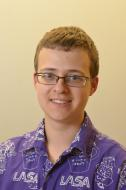
\includegraphics[width=0.2\linewidth]{arthur}
\end{figure}
\subsubsection{Arthur Pachachura - Junior - Programmer /  Marketing / Notebook} 
{\bf My role on the team}: Programmer, Marketing, Pit, Volunteer Evangelist, etc.

{\bf Why I joined Robotics}: I joined robotics because I loved to program and was pretty good at it, but wanted to do more than just sit and throw code at a screen until something worked.  I wanted to work with both hardware and software in one environment.  Now, I'm that plus (apparently) a member of the marketing team.

{\bf What career/job/studies I intend to pursue}: I wish to pursue a career in computer engineering, computer science, and business (entrepreneurship).

{\bf Thing I enjoy most about Robotics \& FIRST}: I never expected to do anything with the marketing department on our team.  Ever.  In fact, my first year, I would have rather used a drill than work on the notebook.  Now, I'm actually enjoying the marketing team.  I get to be one of the first to program an FTC notebook and hope that my product would be used for other teams' notebooks, too.

\begin{figure}[H]
	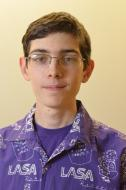
\includegraphics[width=0.2\linewidth]{daniel}
\end{figure}
\subsubsection{Daniel Teal - Senior - Design / Build} 
{\bf My role on the team}: I'm the design/build lead. I make the robot work and then do anything and everything needed to keep it that way. It's a huge time commitment that's definitely worth it.

{\bf Why I joined Robotics}: Before I joined an FTC robotics team, I was pretty good at software development. But code doesn't move physical things very well. Robots, on the other hand, do just that. It was high time for me to get into hardware.

{\bf What career/job/studies I intend to pursue}: I'll earn my master's in MechE, then work in industrial R\&D focusing on automated manufacturing.

{\bf Thing I enjoy most about Robotics \& FIRST}: I love to make wild ideas a reality. Where else besides FIRST would I build a leafblower from scratch? I really enjoy making things work.  

\begin{figure}[H]
	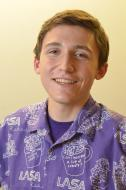
\includegraphics[width=0.2\linewidth]{marek}
\end{figure}
\subsubsection{Marek Travnikar - Senior - Design / Build} 
{\bf My role on the team}: FTC Builder/Designer 

{\bf Why I joined Robotics}: I first joined robotic's mostly because my parents said I should, despite my lack of interest in a club about Lego NXT kits or VEX kits. However, when I say the display FRC 418 had at our school Club Day, I was blown away by the sheer size and complexity of the robots - they were like nothing I had ever seen before (and that says a lot). At that moment I knew this was what I wanted to do in high school, signed up right then, and have remained ever since.

{\bf What career/job/studies I intend to pursue}: I know I want to pursue a job in a field relating to robotics engineering. I know this because everything I have done in the past 3.5 years is the kind of stuff I want to do for the rest of my life. Sure there will be more boring parts here and there, but there will be parts that will be so much cooler, even to the extent of being life changing on a grand scale, I want to be a part of that.  But building robots is only part of it. Over the last few years I have come to quite the leadership position on the team, and realized that perhaps being a leader in the workforce is something I should strive for as well. This is why, in fact, in addition to an engineering degree I fully plan to pursue an education in business, in the hopes it will lead to a place of leadership in my career too.

{\bf Thing I enjoy most about Robotics \& FIRST}: While the taste of victory is sweet, I have found the competition environment prior to be sweeter. Nowhere else have I been able to meet so many people into the same things I am into, so many amazing feats of engineering, and so much of an upbeat atmosphere all in one place. It really is one of a kind and something I really enjoy. 

\clearpage
\newpage

\section{Outreach Overview}
The LASA Robotics Team is committed to outreach.  Comprised of 76 team members from 2 FTC teams (FTC 4290 and 5998 and FRC418) we support various organizations focused on STEM and are key FIURST volunteers in and around Austin, TX.  This year, we were very active, participating in {\bf 38 outreach events} reaching {\bf over 32K attendees}.  Our students are proud that we have logged {\bf over three thousand volunteer hours} from our students, mentors, parents and alumni.   Organizations interested in promoting STEM contact us and our team members step up and help with various demos and outreach programs throughout Central Austin.  A summary of our outreach season is in Table 1 below. \\

\begin{figure}[H]
	\centering
	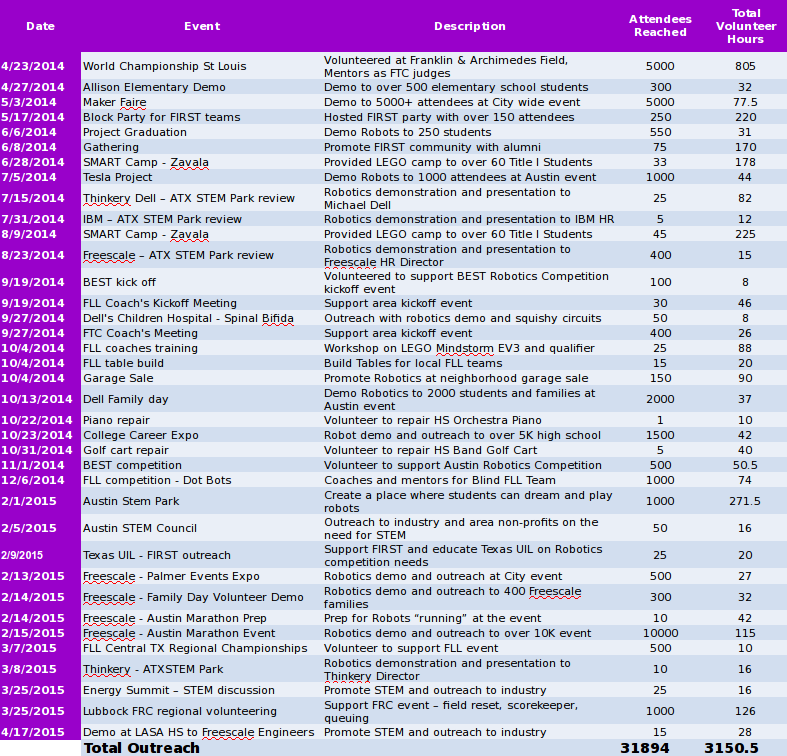
\includegraphics[width=0.9\linewidth]{outreach}
	\label{fig:outreach}
\end{figure}
\begin{figure}[H]
	\centering
	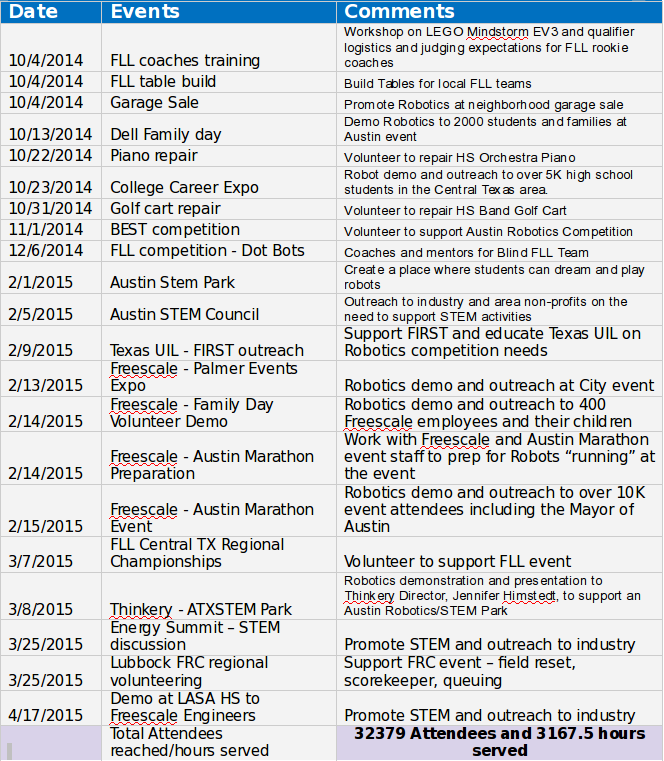
\includegraphics[width=0.9\linewidth]{outreach1}
	\label{fig:outreach1}
\end{figure}

\subsection{In pursuit of a Robotics Park – the ATX STEM Park}
Our goal is to expand access to robotics and STEM in our community. We are working with the City of Austin, industry and Austin Community College to create a permanent Robotics/STEM space in Austin – an intellectual rec center.   This year, we have a temporary space where we were able to stand up half of an FRC field to support this year’s game for practice and testing and host FTC scrimmages.  Our goal is for a permanent and accessible Robotics/STE Park that provides free practice space for all FIRST teams, FRC, FTC and FLL.

\begin{figure}[H]
	\centering
	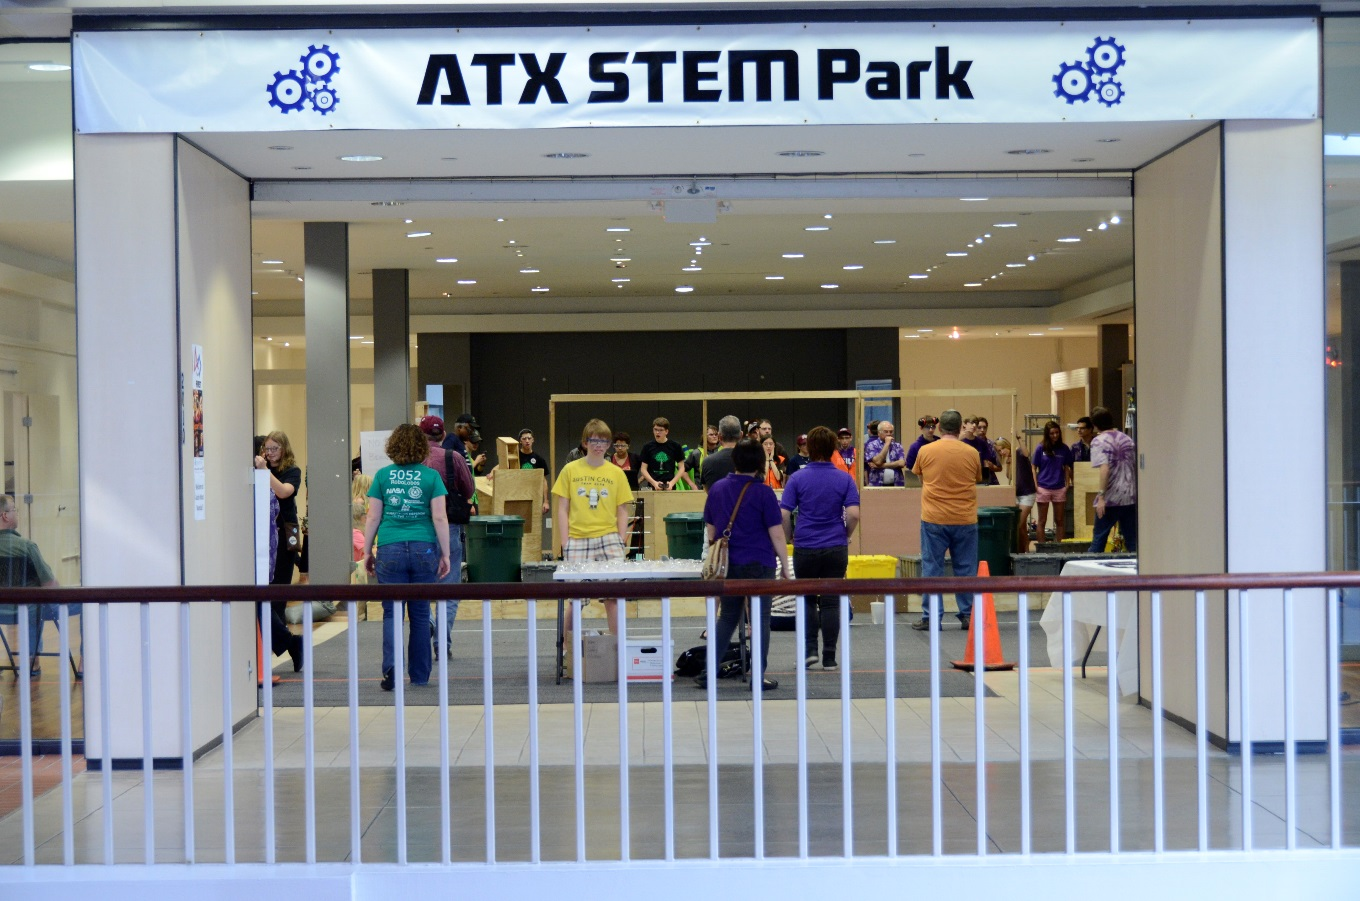
\includegraphics[height=0.9\linewidth]{stempark}
	\caption[]{Austin ATX STEM Park – Highland Mall Entrance}
	\label{fig:stempark}
\end{figure}
\begin{figure}[H]
	\centering
	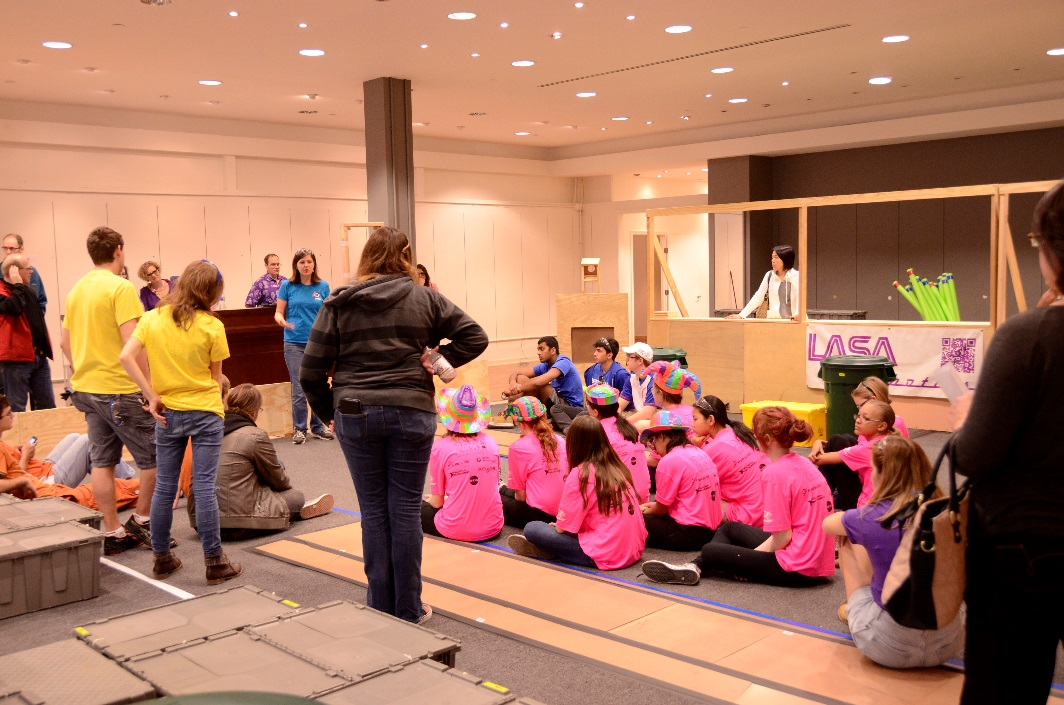
\includegraphics[height=0.7\linewidth]{arr}
	\caption[]{Austin Robot Roundup with local FRC teams}
	\label{fig:arr}
\end{figure}
\begin{figure}[H]
	\centering
	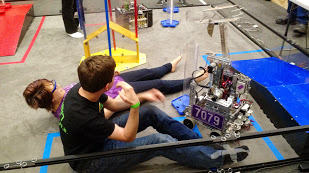
\includegraphics[height=0.7\linewidth]{fridaynight}
	\caption[]{Friday Night Robots with the FTC community}
	\label{fig:fridaynight}
\end{figure}

\subsection{Volunteering at FIRST Events}
To support FLL and FTC programs in central Texas, our team continued to volunteer in FLL and FTC competitions, supplying judges, referees and logistical support.\\

At FLL competitions, we serve as referees, judges and logistical support. At FTC competitions, we are well-known for being a “go-to” resource and problem solvers; our FTC members even help other teams in the challenge box. For FTC and FRC competitions, we give out peer awards to encourage other teams. This season, FTC 7079 and their school superintendent recognized LASA Robotics as the Gracious Professional team they hope to emulate.\\
 
At FLL-focused events and competitions, we provide FTC demos to encourage students to consider progressing to the FTC program. At our family outreach events, including Formula 1, Fun Fest, MakerFaire, Dell Family Day, Freescale events and others, we have demonstrated  FTC and FRC demos to over 46K people in the past 2 years, exciting students about STEM and encouraging participation in FIRST.\\

\subsection{Volunteering at 2014 FIRST World Championship – “Star Volunteers”}
This year, we have been very active and kicked off the season with 3 of our team members volunteering at the World Championships on the Franklin and Archimedes Fields and two of our mentors volunteering to judge the FTC competition at World Championships. Our team members, Arthur and Julia both received the “Star Volunteers” award for their respective fields, an honor for our team and reflective of our commitment to volunteering for FIRST.
\begin{figure}[H]
	\centering
	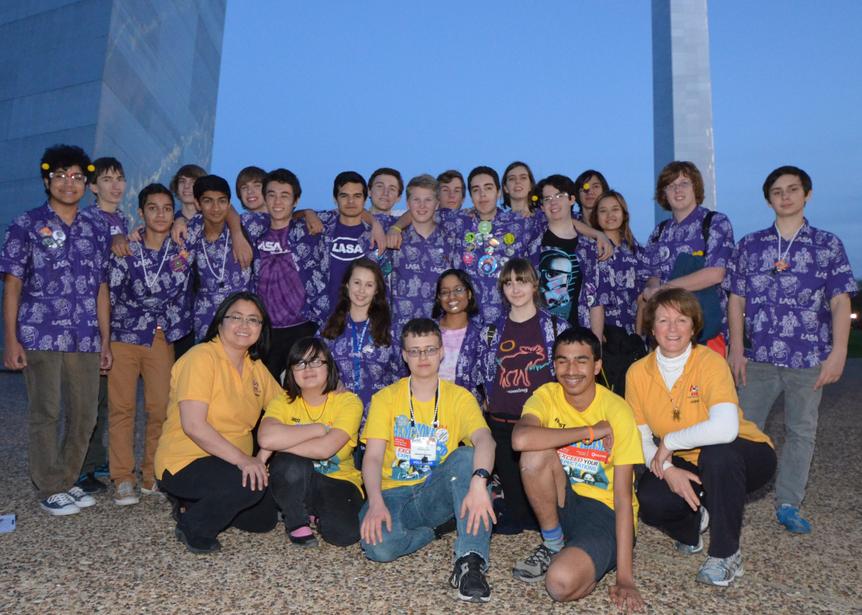
\includegraphics[height=\linewidth]{volunteers}
	\caption[]{Our 2014 World Championship volunteers in yellow shirts}
	\label{fig:volunteers}
\end{figure}

\subsection{SMART Camps}
We continued our support and hosted SMART (Science, Math and Robotics Technology) Camps.  This is our 8th year supporting this program to encourage and stimulate STEM thinking using LEGO Mindstorms to solve a challenge.  We held several camps at Zavala and Wooten Elementary schools, both underprivileged, Title I schools in Austin, TX.\\
\begin{figure}[H]
	\centering
	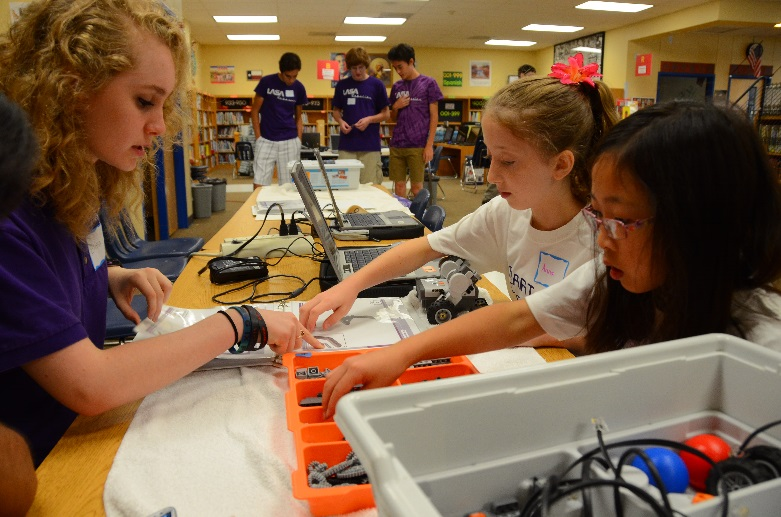
\includegraphics[height=0.8\linewidth]{smart}
	\caption[]{Zavala Elementary School SMART Camp}
	\label{fig:smart}
\end{figure}
\begin{figure}[H]
	\centering
	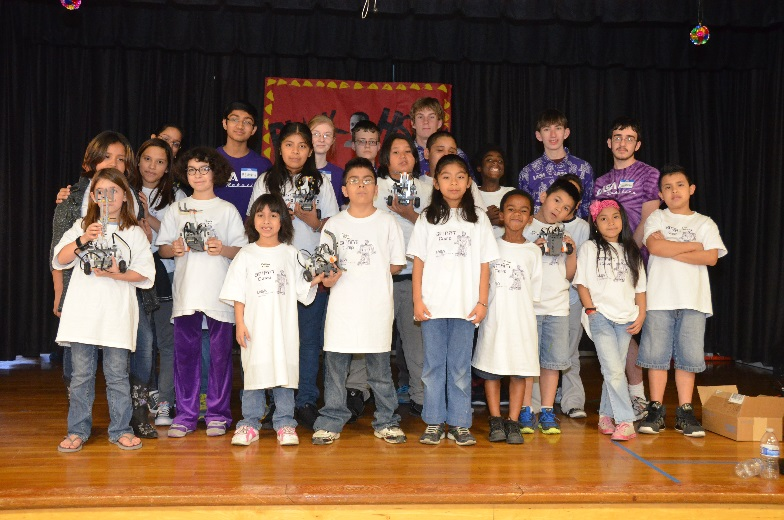
\includegraphics[height=0.8\linewidth]{smart1}
	\caption[]{Wooten Elementary School SMART Camp}
	\label{fig:smart1}
\end{figure}

\subsection{Mentoring the "Dot Bots" - a blind and visually impaired FLL team}
Our LASA Robotics SMART Camps introduce FLL to Title I and other schools, inspiring them to start teams. Through this camp, we recruited enough interest at the Texas School for the Blind to start the “DOT BOTs”, one of the first Blind FLL team in the world. 
\begin{figure}[H]
	\centering
	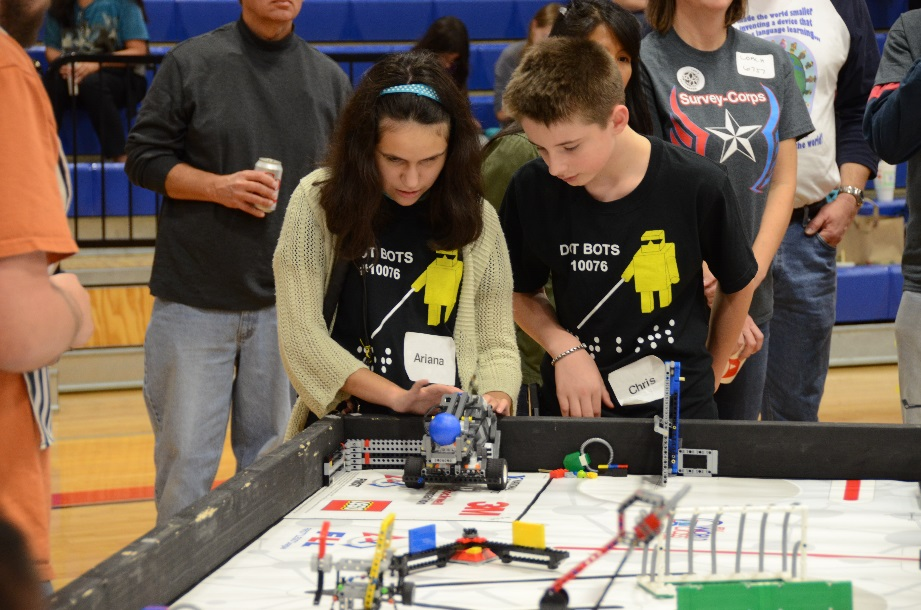
\includegraphics[height=0.8\linewidth]{dotbots}
	\caption[]{Dot Bots at the Hill Country FLL Qualifier}
	\label{fig:dotbots}
\end{figure}

\subsection{Building FLL tables to support FLL teams}
Using our fabrication skills, we have built over 25 regulation FLL Tables for area teams and competitions.   We help teams that don’t have the resources or skills and even deliver these tables to their schools or private homes.  Our tables are high quality and used by Central Texas FLL for the Annual championship competition.
\begin{figure}[H]
	\centering
	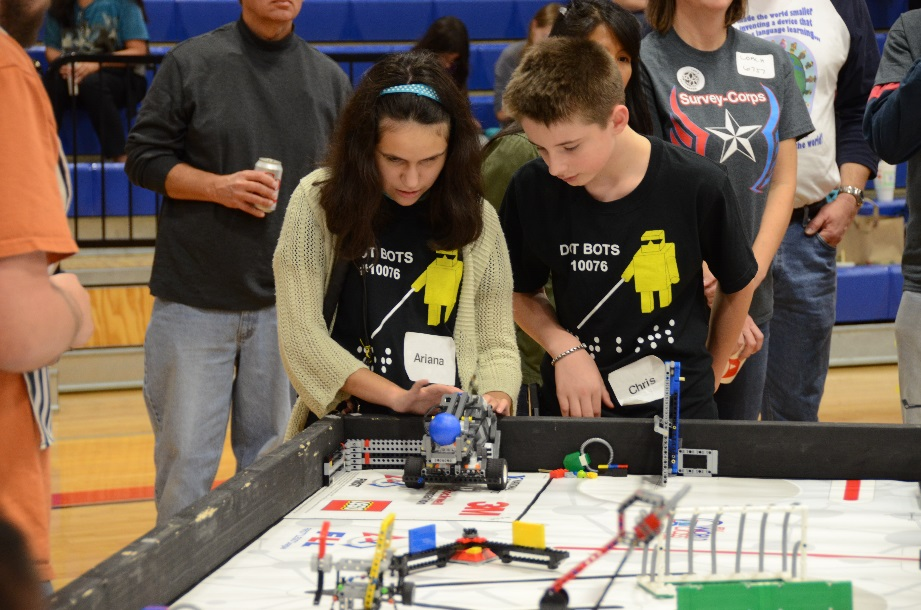
\includegraphics[height=0.8\linewidth]{tables}
	\caption[]{FLL Table build}
	\label{fig:tables}
\end{figure}

\subsection{FLL Rookie Coaches Workshop}
Central Texas FLL has been growing over 20\% every year.  LASA Robotics recognized the need to not only to encourage students to pursue STEM interests and join FLL teams but that we need to increase the number and quality of coaches.  To help increase the confidence of Rookie coaches, one team member created a Rookie Coaches Workshop as his Eagle Project and LASA Robotics piloted this workshop for the first time this September to help coaches learn the new EV3 programming.   Our team mentors, experienced in running FLL qualifiers reviewed the qualifier logistics to provide coaches with a better understanding of how to prepare for competitions.  Two parents on our team who were experienced FLL judges reviewed the scoring rubric to help these rookie coaches understand the expectations at the qualifiers and help better prepare their teams.  Over 20 rookie FLL coaches attended this pilot session and a survey after the workshop indicated overwhelming to offer this workshop of other coaches.
\begin{figure}[H]
	\centering
	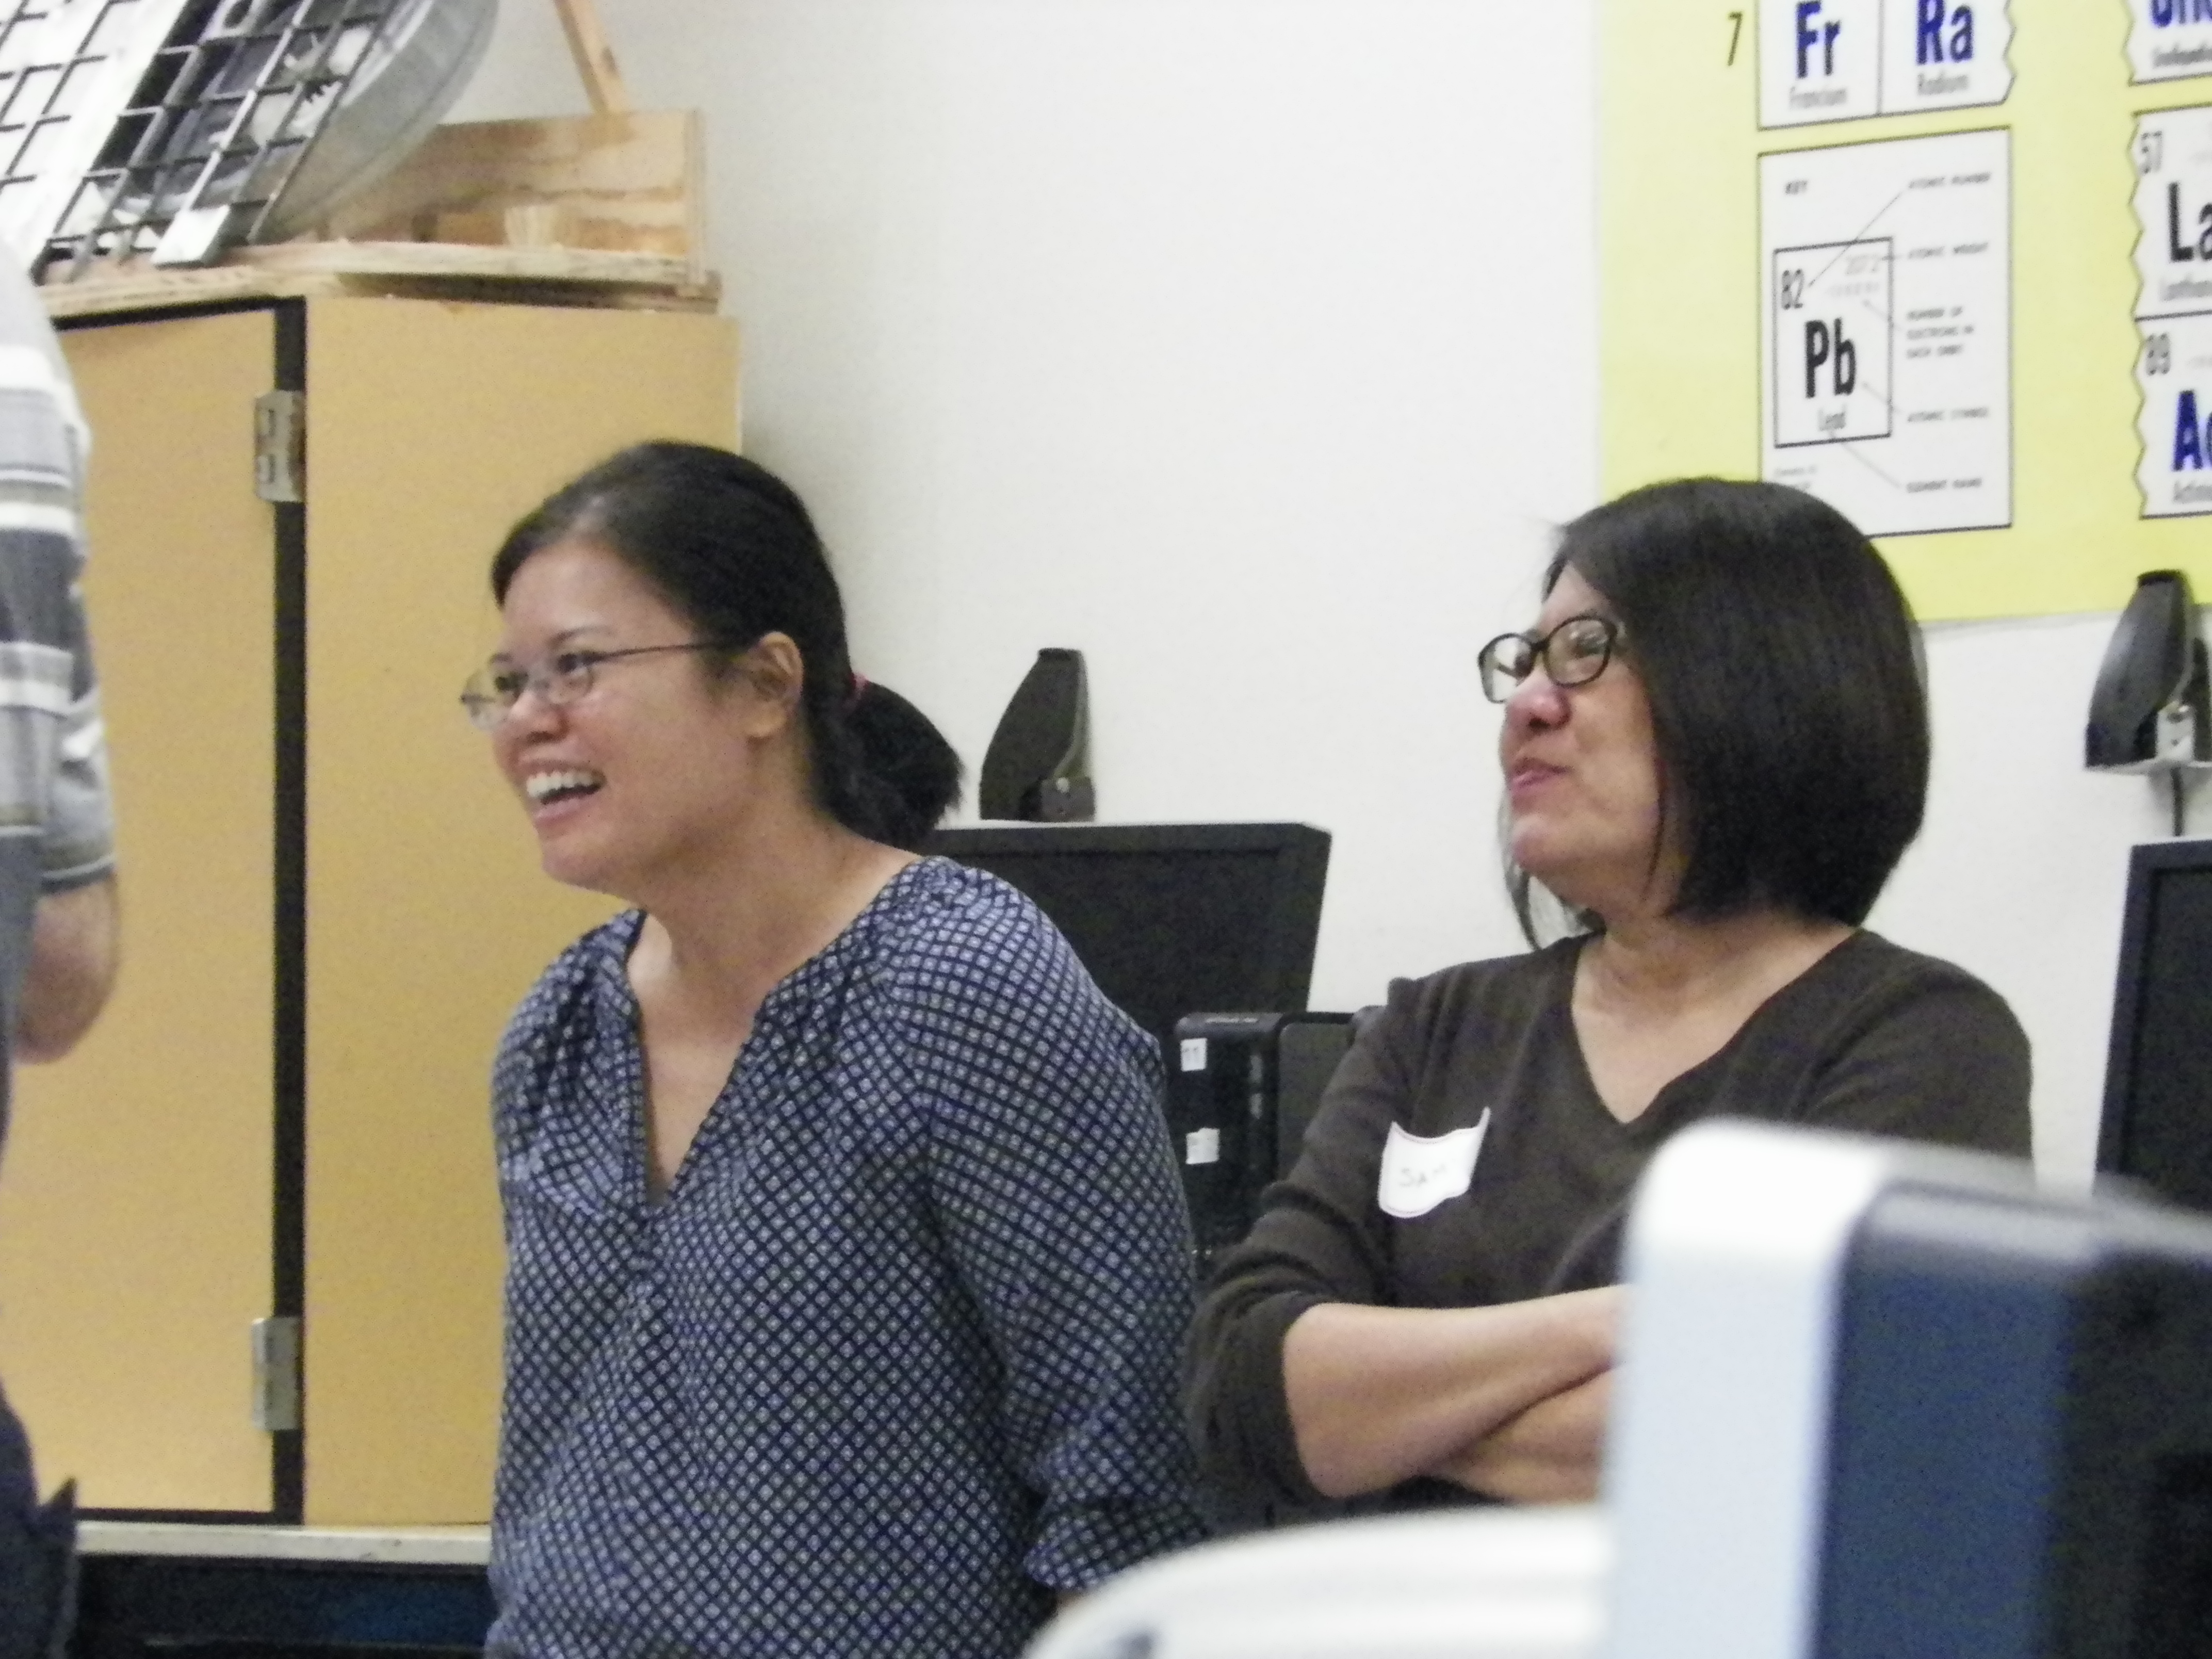
\includegraphics[height=0.8\linewidth]{fll}
	\caption[]{Training workshop for Rookie FLL Coaches - Technical portion}
	\label{fig:fll}
\end{figure}
\begin{figure}[H]
	\centering
	\includegraphics[height=0.8\linewidth]{fll1}
	\caption[]{Training workshop for Rookie FLL Coaches - Core Values portion}
	\label{fig:fll1}
\end{figure}

\subsection{Building the FIRST Community}
We host an annual gathering inviting all area FTC and FRC teams to join and build community.  This season, we had over 150 FIRST participants join us for a fun day of food, festivities and friendly outdoor games.
\begin{figure}[H]
	\centering
	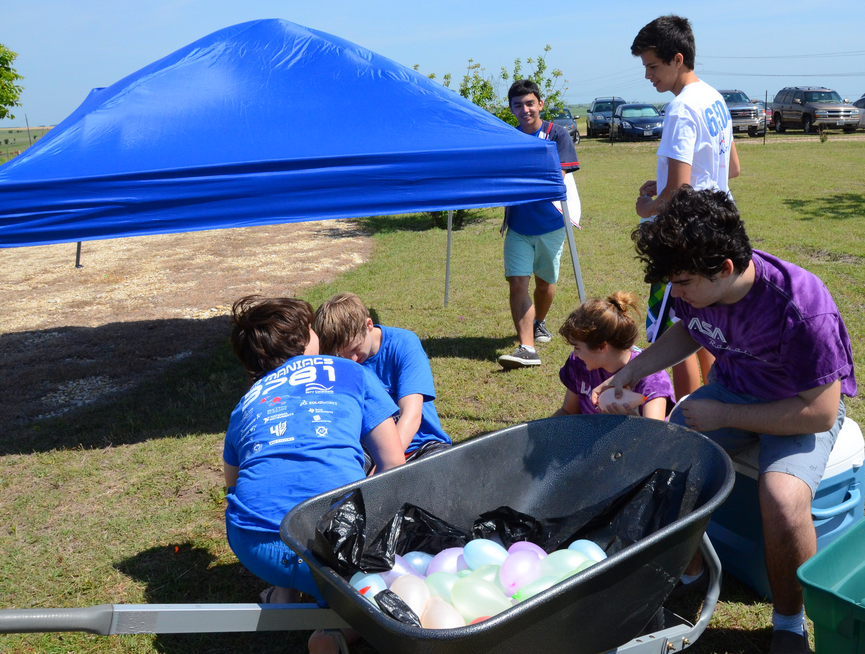
\includegraphics[height=0.8\linewidth]{community}
	\caption[]{Getting ready for a FIRST water balloon fight}
	\label{fig:community}
\end{figure}
\begin{figure}[H]
	\centering
	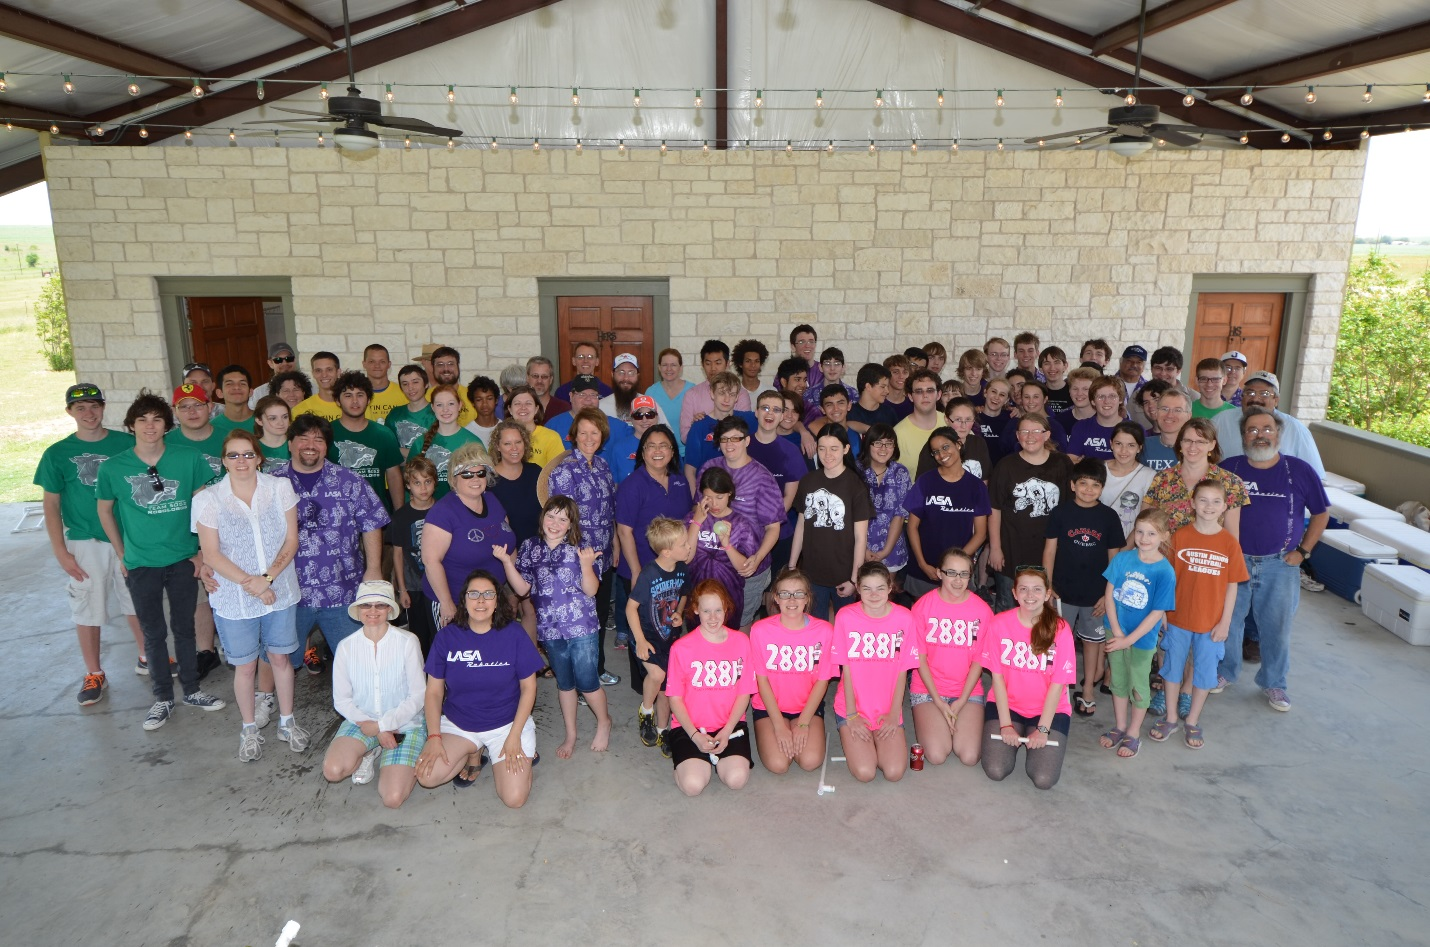
\includegraphics[height=\linewidth]{community1}
	\caption[]{2014 FIRST Block Party }
	\label{fig:community1}
\end{figure}

\subsection{Supporting STEM and FIRST in Texas}
We’re working with FIRST president Don Bossi to engage industry leaders and state legislators to recognize STEM and robotics as a Texas UIL approved extracurricular academic activity, which will impact more than 1200 districts with more than 5 million students statewide.  Our mentors participated in a roundtable hosted by Texas UIL to advocate for FIRST competitions and work to understand how to create a Texas State Robotics Championship.

\section{Business Plan}
\subsection{Team Sustainability LASA Robotics Association}
The LASA Robotics Association is the key to the financial sustainability of the LASA Robotics Team.  The Association is comprised of parents and supporters of the LASA Robotics Team.   We have a president, vice-president, treasurer, secretary and executive director.  In addition, we have 3 parent representatives that participate in decisions.  We hold monthly meetings that are attended by the team coach, team mentors and a student representative. We abide by a set of by-laws that govern the Association’s operations.\\

To help with managing the team operations, we plan an annual budget. We have a documented financial process for team expenditures. The Association requires expenses be authorized through the budget process and any expenses exceeding the budgeted amount must be approved by the board. The treasurer presents a monthly report and only 4 people have check signing authorization at any time. In 2012, an independent bookkeeper completed an audit of our finances and no discrepancies were identified. For the 2014-2015 season, our budget is \$45,750.  See attached budget at the end of the Business Plan Section.\\

To help raise funds, we rely on grants, solicitation of funds from our family, friends and local businesses (ASK) and other fundraisers including paid Robotics Camps (SMART Camps), building FLL tables and selling handmade robotics jewelry.  To help with grants, we have a documented grant process where we seek and identify sponsors to help support the team. In the past 6 years, we have not had any issues with recruiting parents to join the LASA Robotics Association.

\subsection{Fundraising}
For this season, the team and the LASA Robotics Association executed on our plan to improve our financial position.

\subsubsection{ASK Fundraiser}
Our ASK fundraiser has traditionally raised between \$5-\$7K with about 60\% participation.  Our team is now requiring that all students participate in the ASK fundraiser as a condition of travel to increase the participation rate and the total amount raised.  This year, with the growth on our team, we have raised over \$15K with the ASK Fundraiser.  We recognize those family, friends and businesses who respond to our ASK fundraisers by sending them a personalized thank you note along with a picture of the team in action. 

\begin{figure}[H]
	\centering
	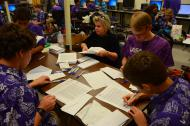
\includegraphics[height=0.3\linewidth]{ask}
	\caption[]{ASK Fundraiser}
	\label{fig:ask}
\end{figure}

\subsubsection{Grants}
We actively recruit parents to specifically help write grants.  We created and updated a grant strategy to pursue grants starting from the summer.  Instead of working with one or two parents and training them to do this, we put together a boilerplate for grant responses so that more parents can quickly get on board and help apply for grants.  Our grant strategy outlined a process where we focus our applications to companies that are already supporting FIRST Robotics.\\

This year, we were successful at applying for and receiving grants and doubled our grants from the previous year to over \$15K for our FRC and FTC teams.  We were very fortunate that the FIRST in Texas Foundation was able to help us with generous re-grants that they solicited from 3M, Texas Workforce Commission, Dell and Freescale.\\

Many long-term sponsors continue to support us with grants: 3M, NI, Time Warner, Texas Workforce Commission, BAE and Smallworks.  Two new sponsors joined last year: Intuitive Surgical and Altera. This year, we added Freescale and DELL.  We strive to maintain long-term, mutually beneficial relationships with all of our donors and sponsors.  At the end of each season, we hold a sponsor’s recognition event where we invite the team sponsors to come and see our team in action.  This year, we invited them to come to the STEM park at Highland Mall.  Some of our sponsors, such as 3M, National Instruments and BAE have supported consistently for many seasons.  We send all donors season updates about the team and recognize key sponsors with handmade wood plaques. 

\begin{figure}[H]
	\centering
	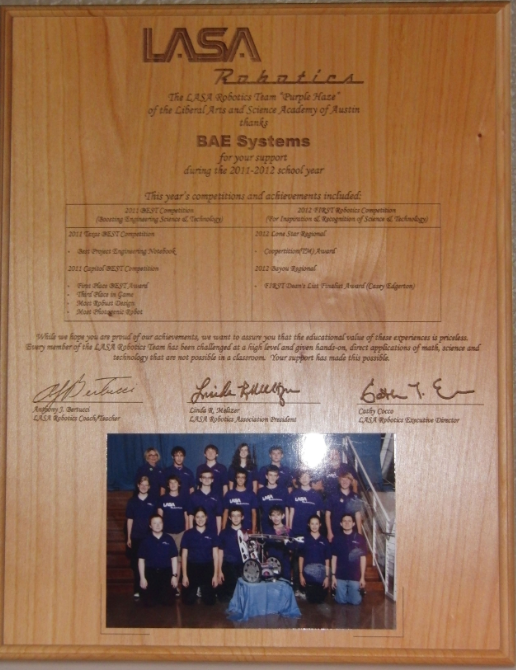
\includegraphics[height=0.3\linewidth]{thankyou}
	\caption[]{Handmade Oak “Thank you” Plaque}
	\label{fig:thankyou}
\end{figure}

\subsubsection{Sponsors}
This year, our sponsors and partners were very generous and enabled us to design and build the best robots we could and help outreach to even more students than ever.  Table 2 lists this year’s LASA Robotics Team Sponsors.

\begin{figure}[H]
	\centering
	
\includegraphics[height=0.3\linewidth]{sponsors}
	\caption[]{2014-2015 LASA Robotics Team Sponsors}
	\label{fig:sponsors}
\end{figure}

\subsubsection{SMART Camps}
LASA Robotics created the SMART Camp (Science, Math and Robotics, Technology) to help spread interest in Robotics and STEM.  Using the LEGO Mindstorms kits, we provide a challenge for students to build, program and have fun with Robots. Our students serve as the mentor for these students ages 8-13.  We provide a SMART Camp T-shirt and a healthy snack to all participants.  These camps have served over 1000 students in the Austin area in the past 6 years, some of whom are currently members of the LASA Robotics Team.  We use these SMART Camps as both for outreach and as a team fundraiser. The outreach camps serve Title I schools and the Texas School for the Blind and Visually Impaired.  We apply for Grants with companies such as 3M and Time Warner to provide these camps free of charge to students.  For a fundraiser, we charge students \$40-\$50 for the beginner and advanced.  The team continues to support and provide SMART Robotics Camps to help inspire younger students from all socio-economic areas in Austin. The team and the mentors invite prospective sponsors, students and parents to come visit the robots at school and at our outreach and competition events to get a better understanding of the team and the FIRST program. The team mentors working with Texas School for the Blind and Visually Impaired (TSBVI) coach of the “DOT BOTS” FLL team to submit a paper to the national organization, the Association for the Education and Rehabilitation of the Blind and Visually Impaired, discussing how blind students can successfully participate in the FLL programs.

\subsection{Team Scholarships}
To help enable all students to participate in FIRST Robotics, the LASA Robotics Association has put together a fundraising plan that sets aside support for scholarships. These scholarships are available to students on the team to help with related team expenses. Last year, over \$2000 was given to help support team travel. This year, we are allocating \$3850 to support scholarships.

\subsection{Risk Analysis}
\subsubsection{Team Strengths}
\begin{itemize}
	\item Commitment from our coach and mentors
	\item Our student body possess strong interest in STEM
	\item Educated and engaged parents
	\item Strong and long term relationships with key sponsors
	\item Strong FLL robotics program in feeder schools
	\item Student lead team
\end{itemize}

\subsubsection{Team Weaknesses}
\begin{itemize}
	\item Need more industry mentors to support team in electronics and public relations
	\item Our coach is within retirement age
	\item School and District provide limited support
\end{itemize}

\subsubsection{Team Opportunities}
\begin{itemize}
	\item FIRST is gaining momentum
	\item Industry Sponsors are becoming more committed to STEM
	\item City and State are interested in making Texas a knowledge economy
\end{itemize}

\subsubsection{Team Threats}
\begin{itemize}
	\item Expense of participation in FRC program
	\item Loss of Industry sponsorships if the economy stalls/declines 
	\item Increase in travel costs to competitions
	\item Texas UIL Robotics giving priority access of shop to another school
\end{itemize}

\subsection{Risk Mitigation Plan}
Team must recruit more industry mentors from:
\begin{itemize}
	\item growing pool of team parents
	\item from our industry sponsor companies
\end{itemize}

Team must work with the school:
\begin{itemize}
	\item to identify, recruit and train potential replacement coaches.
\end{itemize}

We must improve public relations by:
\begin{itemize}
	\item highlighting the benefits of having a FIRST Robotics team
	\item lobbying to increase the support provided by the school administration
\end{itemize}

We must increase our fundraising:
\begin{itemize}
	\item because of possible increases in FRC program costs
	\item to help supplement student travel costs to competitions and team scholarships
\end{itemize}

We must increase and diversify our sponsorship:
\begin{itemize}
	\item to mitigate adverse economic effects to one industry sector 
\end{itemize}

\newpage

\section{Budget}
\begin{figure}[H]
	\centering
	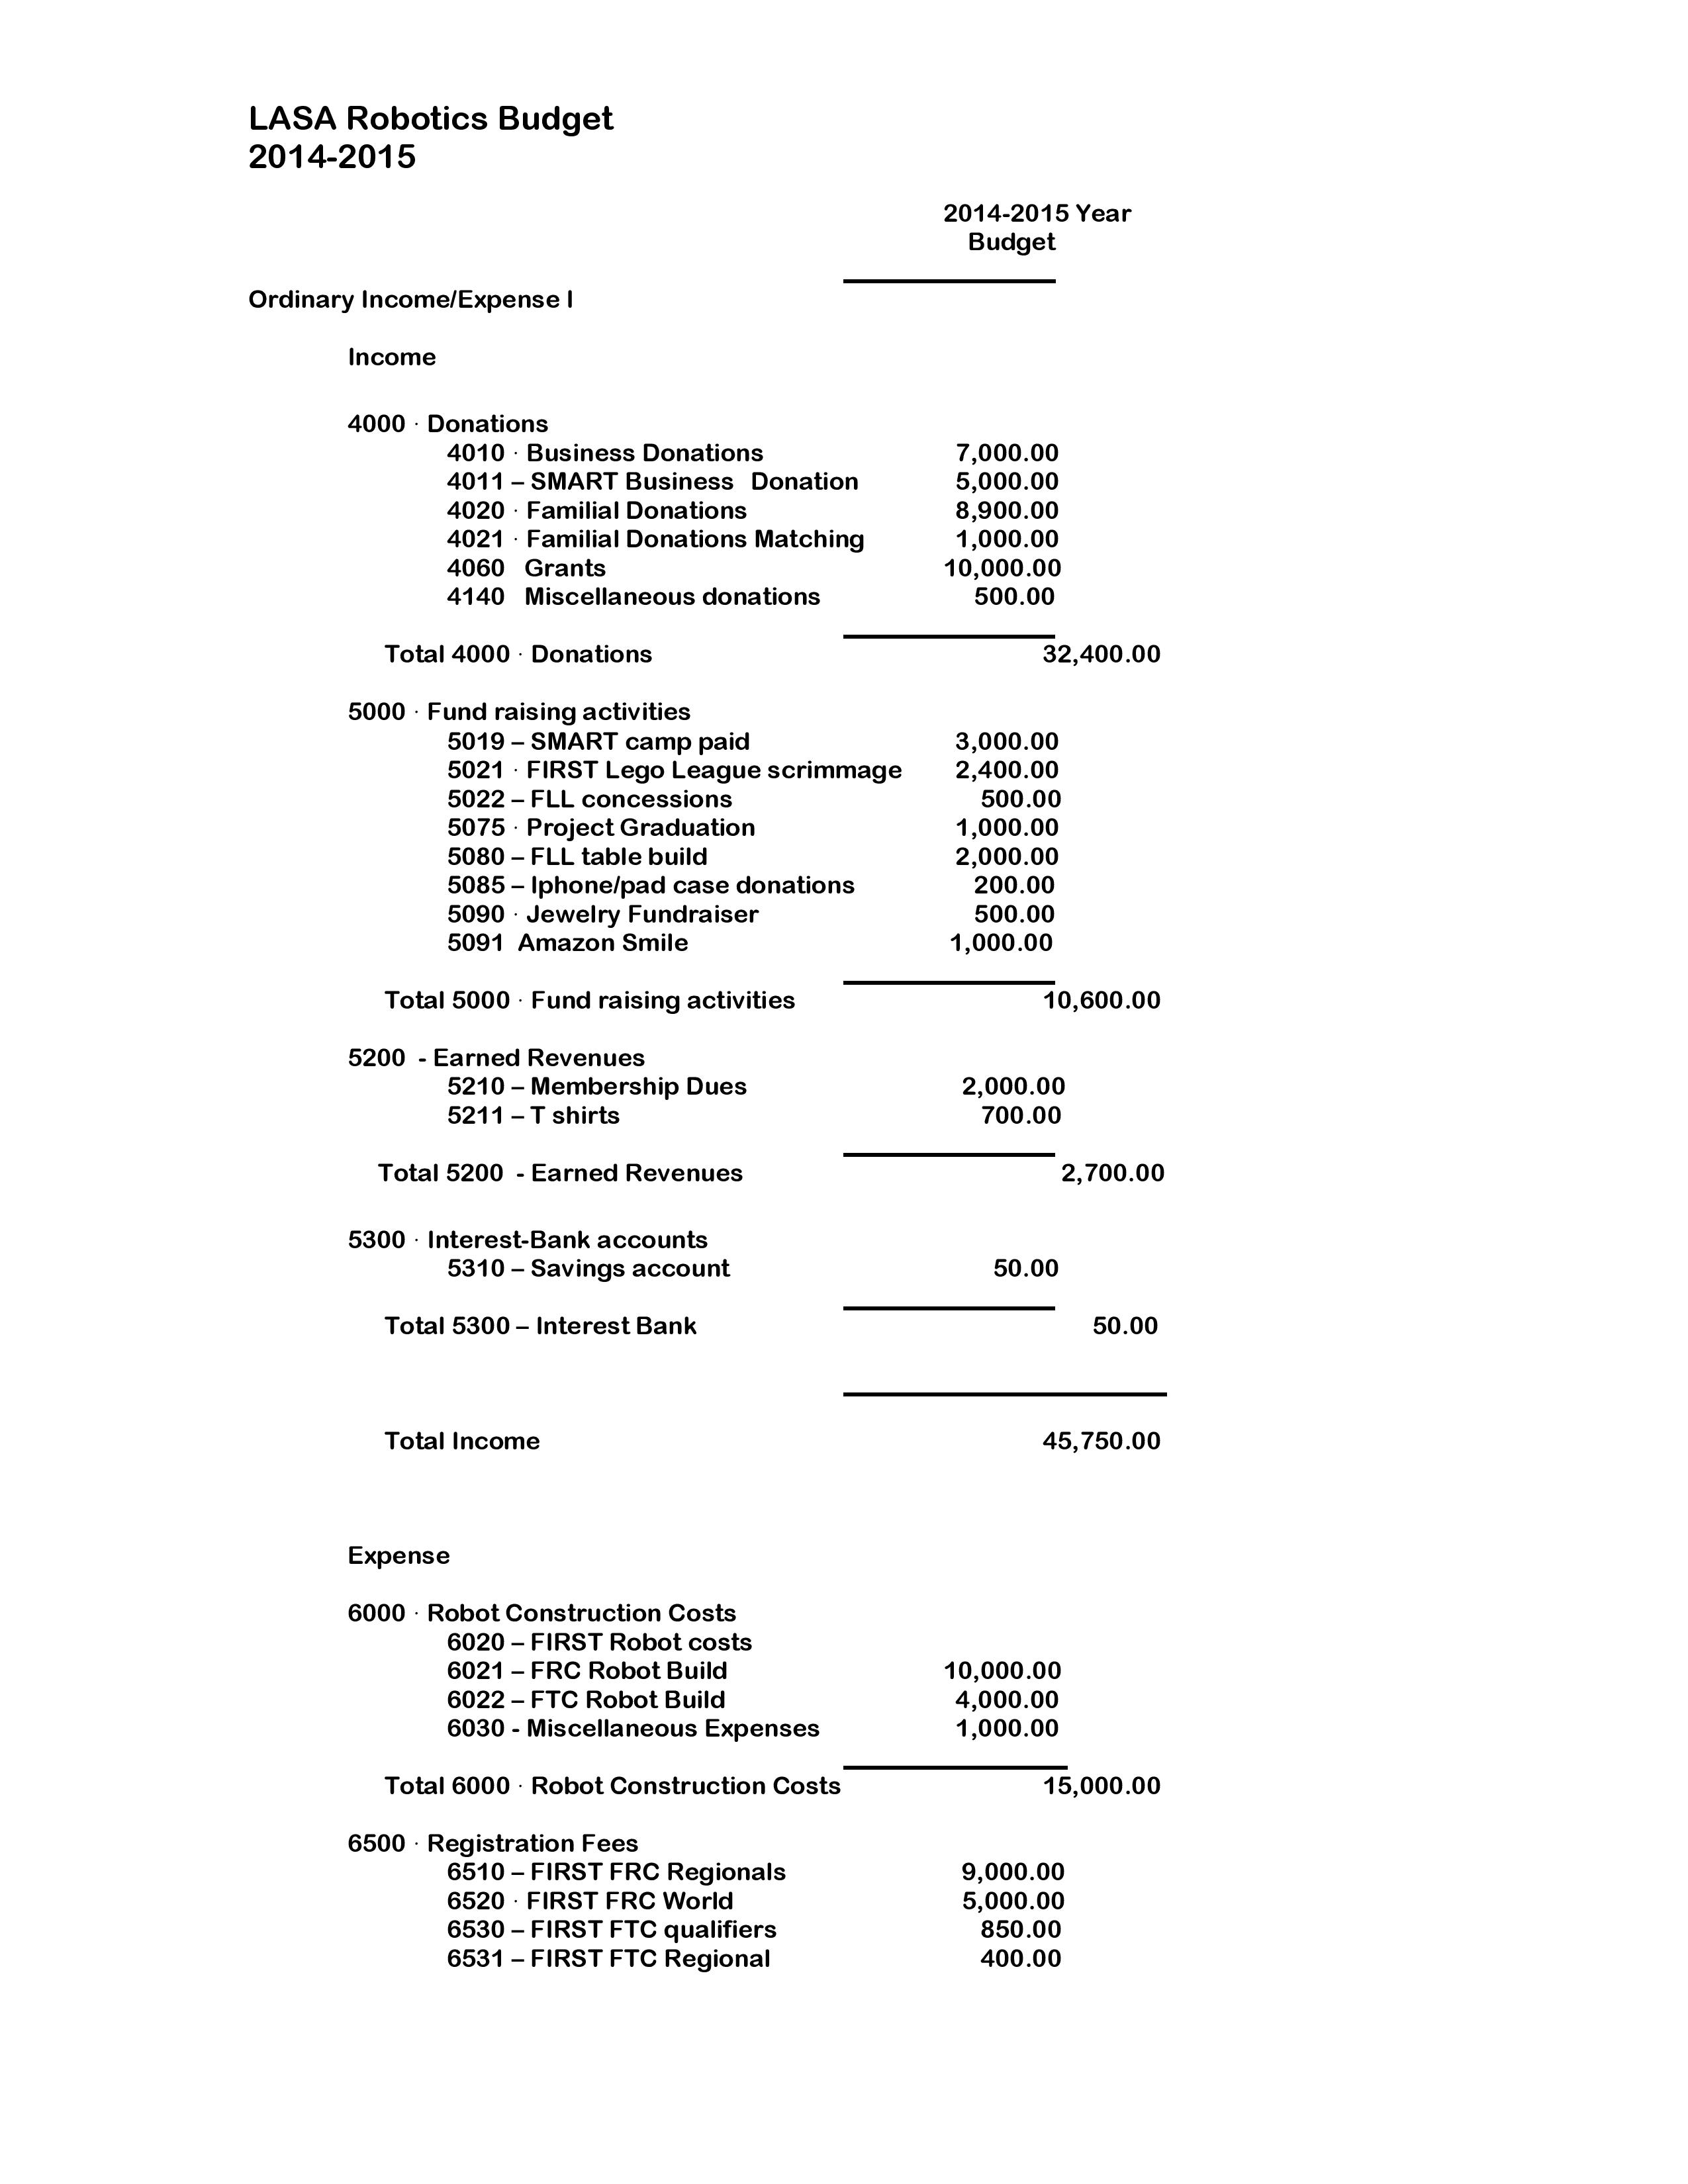
\includegraphics[width=0.9\linewidth]{budget}
\end{figure}
\begin{figure}[H]
	\centering
	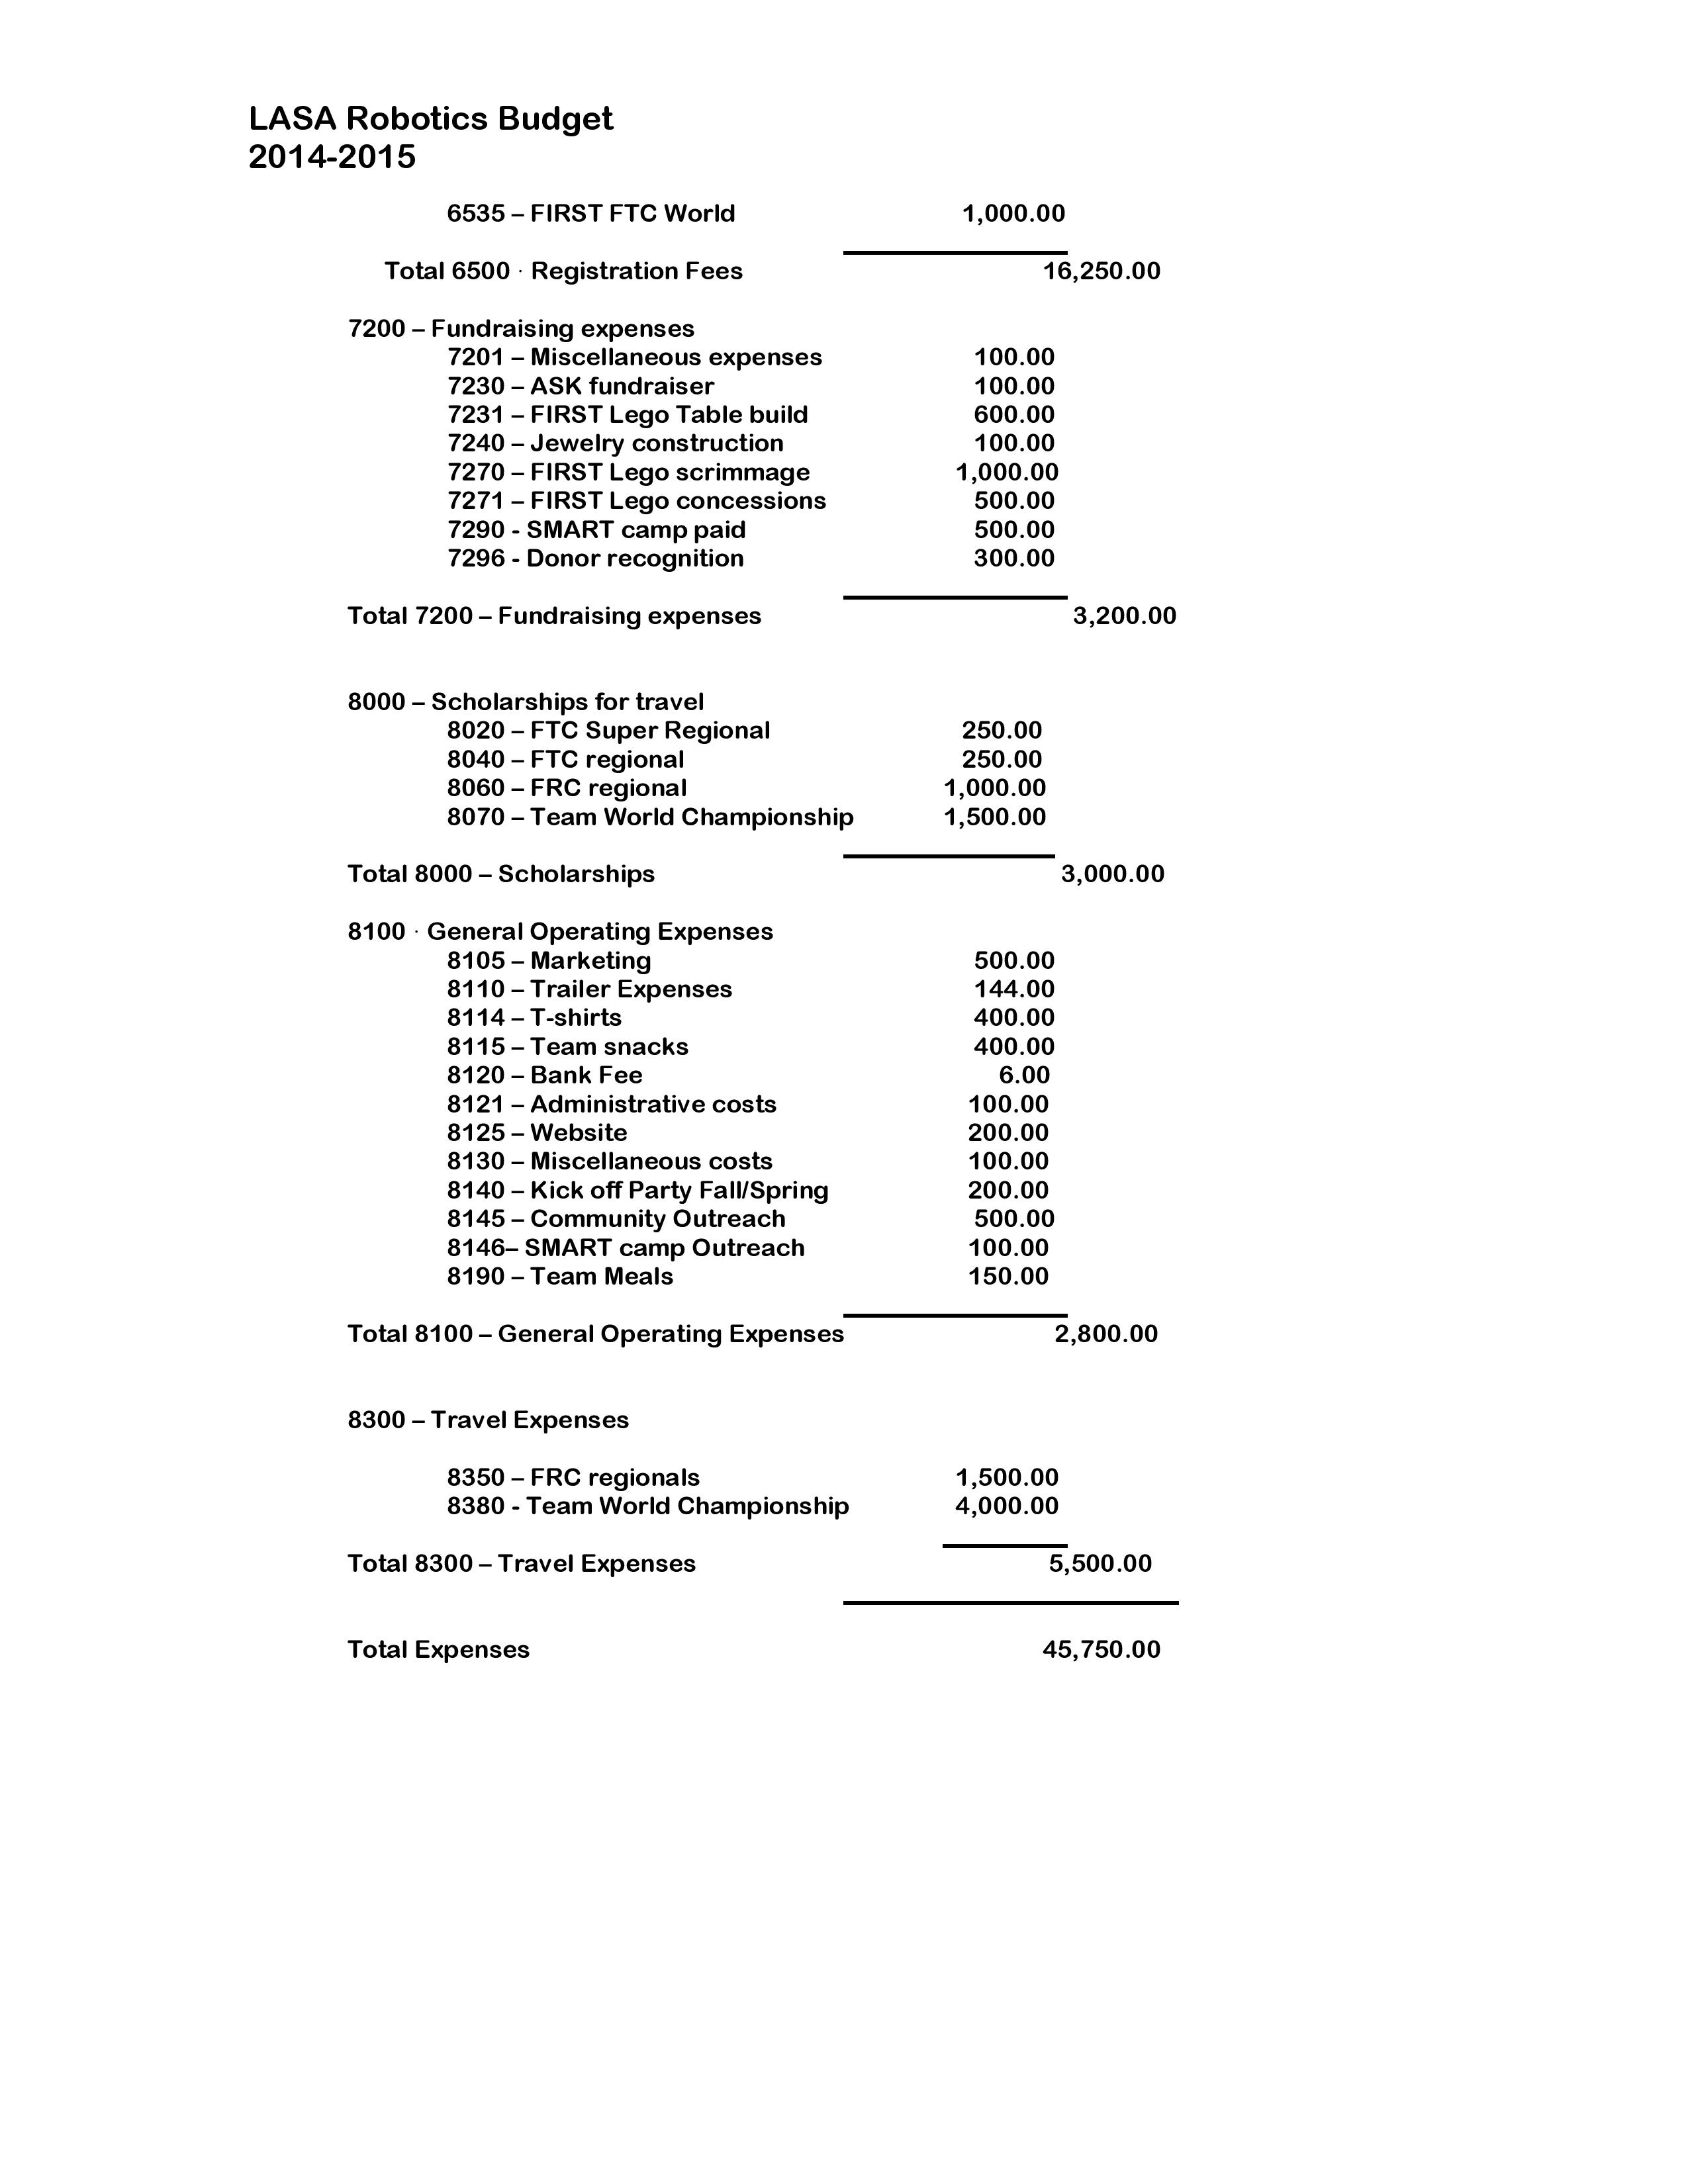
\includegraphics[width=0.9\linewidth]{budget2}
\end{figure}

\newpage
\clearpage
\newpage
\clearpage
\newpage
\color{black}